\documentclass[12pt]{article}
\pagestyle{empty}
\newcommand\tab[1][1cm]{\hspace*{#1}}
\usepackage[margin=1in]{geometry}
\usepackage{array}
\usepackage{amsmath}
%\usepackage{cyrillic}
\usepackage{graphicx}
\usepackage{subcaption}
\usepackage{float}
\usepackage{bm}
\usepackage{tikz}

\thispagestyle{empty}

\begin{document}
\begin{center}
\large\bf Networked Life: Homework 3
\medskip\\
Guo Ziqi - 1000905\\
Zhao Juan - 1000918\\
Zhang Hao - 1000899
\end{center}

\begin{enumerate}

\item{} \textbf{Answer:}\\
\begin{itemize}
\item[(a)] Time the average revenues per click together with the clickthrough rates, we can get the following bipartite graph with the edges indicating values per hour and maximum matching in bold lines:
\bigskip\\
\begin{center}
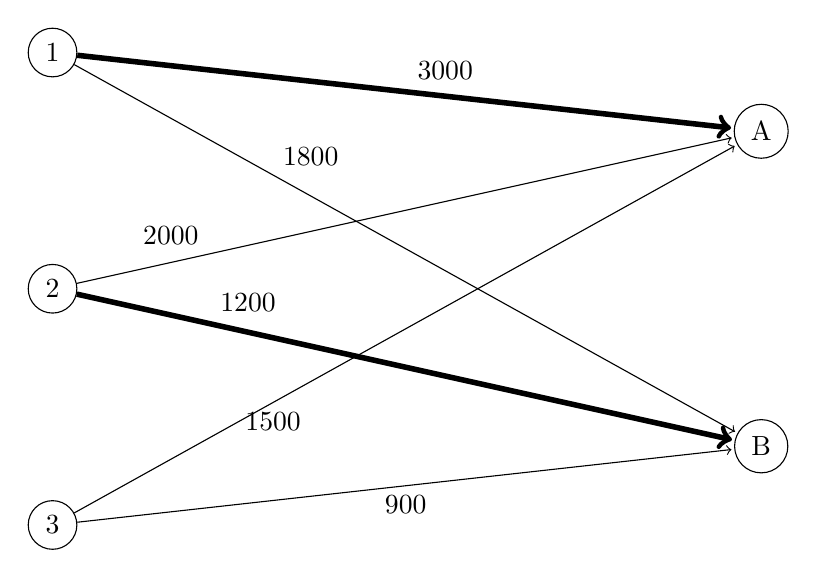
\begin{tikzpicture}
  [->,shorten >=1pt,node distance=3cm,scale=1,auto=left, node_style/.style={circle,draw},edge_style/.style={draw=black}]
  \node[node_style] (n1) at (6,8) {1};
  \node[node_style] (n2) at (6,5) {2};
  \node[node_style] (n3) at (6,2) {3};
  \node[node_style] (n4) at (15,7) {A};
  \node[node_style] (n5) at (15,3) {B};
  \draw[edge_style,line width=2pt] (n1) edge node[pos=0.5]{3000} (n4);
  \draw[edge_style] (n1) edge node[pos=0.3]{1800} (n5);
  \draw[edge_style] (n2) edge node[pos=0.2]{2000} (n4);
  \draw[edge_style,line width=2pt] (n2) edge node[pos=0.2]{1200} (n5);
  \draw[edge_style] (n3) edge node[pos=0.3,below]{1500} (n4);
  \draw[edge_style] (n3) edge node[pos=0.5,below]{900} (n5);
\end{tikzpicture}
\end{center}

\item[(b)] Because $\$6>\$4>\$3$, so ad space A will be assigend to advertiser 1, and ad space will be assigned to advertiser 2.
\medskip\\
The price charged to 1 would be \$4 per click, or $\$4\times500=\$2000$ per hour. The price charged to 2 would be \$3 per click, or $\$3\times300=\$900$ per hour.
\medskip\\
The payoff for 1 is $\$6-\$4=\$2$ per click, or $\$2\times500=\$1000$ per hour. The payoff for 2 is $\$4-\$3=\$1$ per click, or $\$1\times300=\$300$ per hour.
\end{itemize}

\item{} \textbf{Answer:}
\begin{table}[ht]
\caption{Bidding history of all three bidders over reach day of the auction}
\centering
\begin{tabular}{c c c c c c}
\hline\hline
Bidder & Day 1 & Day 2 & Day 3 & Day 4 & Day 5\\ [0.5ex]
1 & (1) 7 & (3) 9.5 & (5) 10$\rightarrow$11 &  & (8) 27.45 \\
2 &  & (2) 9.25 &  & (6) 13.65 & \\
3 &  &  & (4) 9.75$\rightarrow$11.25 & (7) 13.9 & \\
Ask price & 7.25 & 9.75 & 11.5 & 14.15 & 27.7 \\
\hline
\end{tabular}
\label{table: running time}
\end{table}\\
According to the bidding progression, bidder 1 wins the bid and pays \$27.45.

\item{} \textbf{Answer:}
\begin{itemize}
\item[(a)] If $b_1>b_2$, Alice wins the slot with clickthrough rate of 500 per hour. Her payoff is $\$(r-b_2)$ per click, or equivalently, $\$500(r-b_2)$ per hour.
\medskip\\
If $b_1<b_2$, Alice wins the slot with clickthrough rate of 300 per hour. Alice's payoff is then $\$r$ per click, or equivalently, $\$300r$ per hour.
\item[(b)] From the payoffs above, we can equate the two payoffs and find out that when $2/5r>b_2$, getting the first slot will yield higher payoff for Alice; otherwise, getting the second slot will yield higher payoff for Alice. Therefore, the dominant strategy for Alice is to bid $2/5r$, so that in both cases Alice can always maximize her payoff. 
\end{itemize}

\item{} \textbf{Answer:}
\begin{itemize}
\item[(a)] The only scenario that will yield a positive payoff for Bidder 1 is that he wins both seats. However, assuming Bidder 2 is rational, he will always have the choice to give up one seat and bid $\$10$ on the other one. So with a $\$15$ total valuation of the two seats, Bidder 1 would never be able to win both seats.
\medskip\\
In this case, getting only one seat will yield a negative payoff for Bidder 1, as a single seat is worth nothing to him. As the best scenario results in a payoff of $\$0$, not bidding on any of the seats is the dominant strategy for Bidder 1.
\item[(b)] In this case, Bidder 1 just needs to always bid on the package consisting of both seats. Regardless of whether Bidder 2 bids on individual seats or package, Bidder 1 just needs to top Bidder 2's total bid by minimum increment.
\medskip\\
Therefore, Bidder 1 instead can win the bid if package bidding is used. The price charged is $\$(12+m)$ at most, assuming $m$ is the minimum increment to top a previous bid. His payoff is $\$(3-m)$.
\end{itemize}

\item{} \textbf{Answer:}
\medskip\\
The price charged to the winners Bidder 1 and 4 are represented by $p_1$ and $p_4$:
$$M*={(1,1),(4,2)}$$
$$V*=10+9=19$$
$$p_1=(7+8)-9=6$$
$$p_4=(10+8)-10=8$$

\item{} \textbf{Answer:}
\medskip\\
Vector $\pi[k]$ will exhibit periodic behavior as $k$ becomes large. In particular, $\pi[0]=[1/2,1/2,0,0]^T, \pi[1]=[1/2,0,0,1/2]^T,\pi[2]=[0,0,1/2,1/2]^T,\pi[3]=[0,1/2,1/2,0]^T$, and then the pattern repeats itself.
\medskip\\
Therefore, there is no solution for steady-state probabilities $\pi^*$ such that $\pi^{*T}=\pi^{*T}H$.

\item{} \textbf{Answer:}
\medskip\\
When $\theta=0.1$, $\pi_1=0.211, \pi_2=0.205, \pi_3=0.200, \pi_4=0.193, \pi_5=0.190$;\\
When $\theta=0.3$, $\pi_1=0.236, \pi_2=0.221, \pi_3=0.196, \pi_4=0.177, \pi_5=0.170$;\\
When $\theta=0.5$, $\pi_1=0.270, \pi_2=0.249, \pi_3=0.183, \pi_4=0.153, \pi_5=0.145$;\\
When $\theta=0.85$, $\pi_1=0.385, \pi_2=0.369, \pi_3=0.102, \pi_4=0.073, \pi_5=0.071$;
\medskip\\
As $\theta$ increases, the difference of probabilities grows larger. It is more and more obvious that $\pi_1$ and $\pi_2$ have larger significance. This trend is because $\theta$ indicates how much we value the original distribution of transition probabilities. So as $\theta$ becomes larger, the probabilities at equilibrium are mostly determined by the structural connectivity of the graphs.

\item{} \textbf{Answer:}
\begin{itemize}
\item[(a)] $[\pi^*_A,\pi^*_B]^T=[0.827,0.173]^T$
\item[(b)] $[\pi^*_1,\pi^*_2]^T=[0.5,0.5]^T$\\
$[\pi^*_3,\pi^*_4,\pi^*_5]^T=[0.416,0.168,0.416]^T$
\item[(c)] The approximate $\pi^*$ calculated by the given equation is $[0.413, 0.413, 0.072, 0.029, 0.072]^T$.
\smallskip\\
The time complexity of this approximate method is less than that of the directly computing $\pi^*$. No matter if we use inversion or matrices or iterative method, expensive matrix operations like inversion or multiplication is involved. As the matrix dimension $n$ gets larger, computational load would increase exponentially. Splitting the whole matrix into smaller matrices would make computaiton less costly. In this case, updating each iteration would cost around $5^2=25$ multiplications for the original matrix. But once we use the approximation, only $3^2+2^2+2^2=17$ multiplications are needed.
\end{itemize}


\end{enumerate}
\end{document}


 
